\chapter{SOK: Splitting with Oracles and Kappa}
\label{sok}

This chapter describes the combined use of oracles and kappa.
Both techniques are used in the recursive reallocation of work from busy to
idle path processors, referred to as \textit{work splitting}.  The resulting
scheduling technique improves upon the one-time allocation of work used in
breadth-first partitioning by delivering greater speedup and removing the requirement
for accurate selection of a depth limit parameter.

%%%%%%%%%%%%%%%%%%%%%%
\section{Background} %
%%%%%%%%%%%%%%%%%%%%%%

The use of oracles in the breadth-first partitioning one-time scheduling algorithm is
discussed in depth in Chapter \ref{bfp_depth}.  The alternative parallelisation primitive
\texttt{kappa} is covered in Chapter \ref{kappa}.  This section highlights the attributes
of the two approaches exploited in a combined technique to provide effective work splitting.

\subsection{Oracles}
%%%%%%%%%%%%

In the one-time partitioning provided by the breadth-first partitioning strategy
described in Chapter \ref{bfp_depth} and \cite{Sar95}, oracles are used to define subtrees
for search by assigned path processors.  Each oracle is followed to arrive at the root
of the defined subtree, and the depth-first left-to-right execution strategy of standard
Prolog is used within the subtree.  The breadth-first partitioning strategy generates
a complete set of oracles referring to every subtree with its root at the selected
partitioning depth, and the oracles are allocated to the available path processors
such that all the subtrees are searched.

The \textit{current oracle} within a path processor is the sequence of clause indexes
leading to the node in the search tree representing the current point in the
depth-first left-to-right search.
An \textit{open} oracle leads to a choice point
with further branches leading deeper into the search tree.  Generally, the oracles
issued by the depth-first partitioning strategy will be open oracles.

Associated with the scheduling strategy is the concept of \textit{poisoned}
oracles.  If the workload is unevenly balanced among the oracles at the selected
depth limit, one or more open oracles may lead to huge subtrees.  Without work
splitting,  the long runtime of the path processors assigned to those oracles
will dominate the overall runtime and reduce the parallel speedup.  The assignment
of an oracle referring to a very small subtree also reduces the efficiency of the
parallelisation technique, as the path processor will perform the redundant 
computation involved in receiving and following the oracle without then performing
much useful work.  The breadth-first partitioning strategy mitigates the problem
of poisoned oracles by  requiring a partitioning depth at which many open oracles
will be generated, such that the composite workload assigned to each path processor
benefits from averaging.

Oracles have the following useful properties:
\begin{enumerate}
\item{An oracle uniquely identifies a node within the search tree.
  Duplicate solutions can be recognised from their
  identical oracles.  With the one-time assignment of work in the depth-first
  partitioning strategy, duplicate solutions can be found if they appear beneath
  the selected depth limit.  In this case duplicates can be avoided with the
  simple mechanism of limiting those solutions to the path processor given
  a unique processor number $N=0$.  More complex strategies can provide
  speculative assignment of work in the knowledge that duplicate solutions can
  be recognised.}
\item{An open oracle can be treated as a reference to its underlying subtree.
  Another processor can use the oracle to recreate the environment at the root
  of that subtree, and can then independently perform the search of that subtree.}
\item{With each path processor following a strict depth-first left-to-right
  search strategy, an oracle can be considered to divide the search tree into
  two parts, to the left and right of that oracle respectively.  A busy
  processor can return the oracle referring to its current node in the search
  tree.  The implied left subtree represents the part of the tree already searched, while
  the right subtree represents the part of the tree still to be searched.}
\end{enumerate}

\subsection{Kappa}
%%%%%%%%%%%%

The partitioning primitive \texttt{kappa} is described fully in Chapter \ref{kappa}.

The breadth-first partitioning strategy generates all the open oracles at a
selected depth in the search tree, and then distributes all the oracles to the
available path processors.  The path processors then follow each assigned oracle
to search each associated subtree.  To reduce the communications requirements,
\textit{all} the oracles can be generated locally at every path processor, and
each can use the allocation algorithm to select those for local search.

To reduce the overhead of processing the many oracles referring to small
subtrees, the optimal partitioning depth limit will be that at which the number
of open oracles $S$ considerably exceeds the number of processors in the 
group $G$.  Each path processor will be allocated $S/G$ oracles.  For example,
at the optimal partitioning depth $L=21$ for the pentominoes problem, 848
open oracles are discovered for allocation to the 30 path processors, so they
each receive 28 or 29 oracles.

The parallelisation primitive \texttt{kappa} provides the same 
distributed behaviour as the
allocation of the open oracles in the breadth-first partitioning strategy, without
the requirement to accumulate and store the potentially large 
number of open oracles.  The
bounded-depth phase of BFP is interleaved with the search of the assigned
subtrees as each node which would otherwise have generated an open oracle is
discovered.  The recomputation of the path up to the root of the selected subtree
is avoided.

%%%%%%%%%%%%%%%%%%%%%%%%%%
\section{Work splitting} %
%%%%%%%%%%%%%%%%%%%%%%%%%%

The combined support for both oracles and \texttt{kappa} provides an effective
means to interrupt the work of a busy path processor and assign the remaining
work to a newly formed group of idle path processors.  The general idea is
illustrated in Figure \ref{splitting}, in which one path processor is dividing
its work among three others.

\begin{figure}[htb]
\vspace{5mm} \hbox to \hsize{\hfill \psfig{file={sok/ps/splitting.ps}} \hfill}
\caption{Work splitting.}
\vspace{5mm}
\label{splitting}
\end{figure}

This section describes how the parallelisation support has been extended to
facilitate work splitting, and discusses consequent scheduling issues.  
Effective work splitting is dependent upon:
\begin{itemize}
\item{The ability of a busy path processor to efficiently communicate a specification
  of its remaining work to idle path processors.}
\item{The reduction of the remaining work into a number of reasonably balanced
  subtasks.}
\item{The ability of each assigned processor to recreate efficiently the context
  of the allocated subtask such that the work of the interrupted processor can
  be continued and ultimately completed.}
\end{itemize}

Oracles provide effective support for the first and third requirements, while
breadth-first partitioning with \texttt{kappa} is sufficient for the second.

\subsection{At the busy path processor}
%%%%%%%%%%%%

Each path processor maintains the current oracle referring to its current node
in the search tree. On interruption, the busy path processor communicates
its current oracle and aborts the search of the current subtree.  Assuming the
busy path processor has been assigned a current partitioning depth limit $L$,
the processor continues its search with the next allocated subtree at $L$.  The
point at which work splitting is initiated is described (and implemented) 
as an `interruption'. This is to support scheduling strategies in which the interrupt
is generated externally in addition to strategies in
which some internal threshold (such as accumulated choice point count) triggers
the work splitting in the busy path processor.

\begin{figure}[htb]
\vspace{5mm} \hbox to \hsize{\hfill \psfig{file={sok/ps/busy_pp.ps}} \hfill}
\caption{Interruption of a busy path processor.}
\vspace{5mm}
\label{busy_pp}
\end{figure}

\enlargethispage{-\baselineskip}  % manual final formatting
The situation at the busy path processor is illustrated in Figure \ref{busy_pp}.
In the prototype implementation of the splitting with oracles and kappa
(SOK) strategy with
PrologPF the interruption of the busy path processor causes it to:
\begin{enumerate}
\item{Communicate its current oracle to the control processor.}
\item{Reset its state
  to the root of the search tree.}
\item{Continue the partitioning of the search tree at the depth limit $L$, but
  searching to the right of the previous current oracle.  Due to the depth limit
  $L$, the busy path processor need only use the first $L$ indexes of the oracle
  to determine the left bound of the continued search.  This oracle prefix of 
  length $L$ is called the \textit{port oracle}.}
\item{It is possible to interrupt the busy path processor when its current 
  depth is below the
  depth limit $L$, in which case the response to the interrupt is deferred until
  the path processor reaches the next port at $L$.}
\end{enumerate}


\subsection{At the idle path processors}
%%%%%%%%%%%%

A number of idle path processors are formed into a group with a new group
count $G'$, and new unique processor numbers $N'=0\ldots G'-1$.  They are
given the current oracle from the interrupted busy path processor with a
new depth limit $L'$.   The situation is illustrated in Figure \ref{idle_pp}.

\begin{figure}[htb]
\vspace{5mm} \hbox to \hsize{\hfill \psfig{file={sok/ps/idle_pp.ps}} \hfill}
\caption{Assignment of work to an idle path processor.}
\vspace{5mm}
\label{idle_pp}
\end{figure}

On receiving the oracle and the parameters $G'$, $N'$ and $L$ and $L'$, the path 
processor will:
\begin{enumerate}
\item{Follow the oracle to a depth $L$ to arrive at the root of the subtree
  previously partially searched by the interupted busy path processor.}
\item{Use the breadth-first partitioning technique with \texttt{kappa} to
  arrive at each allocated port at the new depth limit $L'$ and search the
  defined subtree.  Throughout this phase, the path processor's search 
  is constrained to the right of the remainder of the provided
  oracle.}
\end{enumerate}

Once executing, the previously idle path processors become busy.
If interrupted, a path processor in the new group 
will return its current oracle and depth
limit $L'$ and the splitting algorithm will be recursively applied.

\section{Scheduling}
%%%%%%%%%%

As described above, PrologPF programs with support for splitting with oracles and
kappa enable any busy path processor to be interrupted and the work divided between
any number of idle path processors.  These capabilities provide a foundation for
a diverse range of scheduling algorithms.  Choices to be made in the scheduling
algorithm include:
\begin{itemize}
\item{The criteria to determine \textit{when} one or more busy path processors should be
  interrupted to redistribute their remaining work.}
\item{How to determine \textit{which} busy path processor to interrupt.}
\item{The size of the new group to receive the divided workload.}
\item{The specification of the incremental depth limit $L'$ for the new group.}
\item{Whether the scheduling decisions should be made locally within the
  busy or idle path processors, or whether more effective scheduling can be
  provided with a control processor.}
\end{itemize}

The importance of efficient scheduling has been recognised in other OR-parallel
Prolog implementations, such as Aurora \cite{Bea91} and Muse \cite{Ali87}. Butler
and others discuss the issues of scheduling on the
ANL-WAM OR-parallel system in \cite{BDLO+88}.
The implementation of the SOK strategy in PrologPF has not so far been used to 
investigate these choices in any depth.  A trivial scheduling algorithm was
embedded into the control processor running \texttt{skynet} (Appendix \ref{skynet}),
with the following characteristics for an initial group of 30 path processors:
\begin{itemize}
\item{A busy path processor will be interrupted when the number of idle path processors
  is $\geq 3$.  This parameter of SOK is called \texttt{split\_{}g}.}
\item{The busy path processor selected for interruption will be that with a current
  partitioning depth nearest the
  root of the problem search tree.  Interruptions occur round-robin for busy path
  processors at the same least partitioning depth.}
\item{The work of the interrupted path processor is assigned to 3 previously idle
  path processors.}
\item{Two techniques to arrive at the incremental depth limit were evaluated:
  \textit{fixed} and \textit{doubling}.  In the former the recursive depth limit
  is incremented by a fixed amount on each splitting of the workload, and in the
  latter the incremental depth limit $L'$ is always double the depth limit $L$
  of the interrupted busy processor.}
\item{Scheduling is managed by a centralised control processor, which 
  receives the completion messages and generates
  the interrupts.
  The interrupted processors communicate their current oracle to the control
  processor, which selects the idle processors for work assignment and
  dispatches the work.}
\end{itemize}

The one-time partitioning of the BFP strategy is analagous
to the SOK strategy with
\texttt{split\_{}g} $> G$, such that no splitting takes place.

%%%%%%%%%%%%%%%%%%%
\section{Results} %
%%%%%%%%%%%%%%%%%%%
\enlargethispage{\baselineskip}  % manual final formatting
For the performance results of the one-time partitioning BFP strategy
in Chapter \ref{bfp_depth}, the
cpu time of the path processors could be used to arrive at the overall runtime.
This removed consideration of the load time of the processes and the communication time
of the solutions.  This simplification was acceptable for a strategy with no
scheduling communication after the intial distribution of the problem.  The
strategy of splitting with oracles and kappa (SOK) involves repeated communication during
the execution of the problem, such that overall real runtime is important in the 
assessment of the scheduling technique.  The runtime for the 
SOK strategy is measured from the point at
which all the path processors are loaded with the sample program to the point at
which all path processors are idle.

\begin{figure}[htb]
\vspace{5mm} \hbox to \hsize{\hfill \psfig{file={sok/ps/zones.ps}} \hfill}
\caption{Interpretation of oracle as dividing search tree.}
\vspace{5mm}
\label{zones}
\end{figure}

From the benchmarks used to evaluate the BFP strategy, the Pentominoes problem has
been used for comparison with SOK in this section.  The SOK strategy is implemented
with three variants of the embedded parallelisation primitive,
illustrated in Figure \ref{zones}:
\begin{enumerate}
\item{\textbf{No oracle partitioning:} the interpretation of an oracle as dividing
  the search tree into two parts is not exploited either above or below the depth
  limit.  After interruption, a busy path processor must restart its search from
  the left-most path in the search tree below the depth limit to arrive at the
  next allocated port to then search the referenced subtree.  On receiving the
  oracle, an idle path processor must fully search the first allocated subtree
  possibly duplicating work within that subtree
  already performed by the interrupted path processor.}
\item{\textbf{Oracle partitioning to ports:} The oracles returned by an interrupted
  busy path processor are truncated to length $L$, such that they refer to the
  current port only.  On interruption, the busy path processor has reset its state
  to the root of the search tree, but can efficiently continue its search by
  ensuring it searches to the right of the oracle leading to the port assigned to
  the idle processors.  The busy path processor thus avoids duplicating the work
  performed in the shaded zone A in Figure \ref{zones}, but the idle path processors
  will possibly duplicate work already performed in the subtree
  with its root at B.  This partial use
  of the interpretation of the oracle as dividing the search tree provides a more
  efficient interrupt handling in the busy path processor, and provides a mechanism
  by which one or more of the idle path processors could efficiently divide the
  remaining work of the busy path processor at the depth limit $L$.  The implementation
  tested here only divides the work of the busy processor within its current
  subtree.}
\enlargethispage{\baselineskip} % manual final formatting
\item{\textbf{Full oracle partitioning:} The full current oracle is returned by a busy
  path processor on interruption (``root to X'' in Figure \ref{zones}).  The busy
  path processor searches to the right of that oracle to arrive at the next allocated
  port, and the idle processors will search to the right of that oracle within the
  subtree, avoiding duplication of work in the shaded area ``B'' in 
  Figure \ref{zones}.}
\end{enumerate}

As real runtime has been used for the SOK speedup figures, the evaluation is
more vulnerable to the load placed on the processors and network by other users.
The results of several runs are averaged to produce the figures used in the
speedup graphs.  The variance was approximately 5\%.

\subsection{Fixed depth increment}
%%%%%%%%%%%%

Figure \ref{spd_compare_fixed} shows the speedup performance for the SOK strategy
with a fixed depth increment
for a range of values of the initial partitioning depth limit $L=1\ldots 30$.  The
speedups for the BFP strategy is included for comparison.  The fixed depth increment
was chosen to be equal to the initial depth limit selected for the problem.

\begin{figure}[htb]
\vspace{20mm} \hbox to \hsize{\hfill \psfig{file={sok/ps/spd_compare_fixed.ps}} \hfill}
\caption{Pentominoes: splitting with fixed incremental depth limit.}
\vspace{5mm}
\label{spd_compare_fixed}
\end{figure}

The area labelled ``A'' in the graph in Figure \ref{spd_compare_fixed}
represents the improvement due to the more
efficient interrupt handling provided in the busy path processor by exploiting the
interpretation of the oracle as dividing the search tree beneath the depth limit
$L$.  Following the interruption the path processor does not then have to redo the
work to the left of the oracle leading to the previous current port.  The area
labelled ``B'' in the graph in Figure \ref{spd_compare_fixed} represents the 
improvement in efficiency resulting from the exploitation of the full oracle to
avoid duplication of work within the assigned subtree.

The SOK strategy with a fixed incremental partitioning depth consistently
outperforms the one-time partitioning of the BFP strategy.  However, with no oracle
partitioning, with the busy path processor resetting to the root of the
search tree on interrupt, and with the simple scheduler implemented in skynet,
the SOK strategy performs badly with large initial values of the partitioning depth
parameter.  For example, with an initial depth limit of 30,
when 3 path processors have become idle a busy path processor will be interrupted,
and the subtree defined by the returned oracle will be partitioned at a depth
of 60.  At this depth there is generally little work to do in the Pentominoes
problem and those processors will quickly become idle, triggering the
interruption of another busy path processor.  As the problem nears completion, path
processors become idle more rapidly than the remaining busy processors can
respond to interrupts, and the system spends more time handling interruptions than
performing useful work. 

With small values for the initial partitioning depth,
the use of the same parameter to provide the incremental partitioning depth
results in inefficient partitioning as at each recursive step only a small number
of ports are found at the new partitioning depth.  The worst case is for $L=1$
where splitting will occur at $L=1$ and then $L=2$ and $L=3$ and so on.  In effect,
the system must split the work of a busy processor several times before an
efficient partitioning is achieved.

\subsection{Doubling depth increment}
%%%%%%%%%%%%
\enlargethispage{-\baselineskip}  % manual final formatting

Figure \ref{spd_compare_doubling} shows the speedup ratios achieved with the
SOK strategy with the incremental depth limit recursively set to
double each previous value. The speedups of the 
one-time partitioning strategy BFP are included for
comparison.

\begin{figure}[htb]
\vspace{15mm} \hbox to \hsize{\hfill \psfig{file={sok/ps/spd_compare_doubling.ps}} \hfill}
\caption{Pentominoes: splitting with depth limit doubling.}
\vspace{5mm}
\label{spd_compare_doubling}
\end{figure}

The area labelled ``A'' in Figure \ref{spd_compare_doubling} 
represents the improvement of the more efficient
interrupt handling provided by the search to the right of the port oracle in the
busy path processor.  This improvement matches that found with the fixed depth
limit incrementing technique.  As with the fixed technique, the area labelled
``B'' shows the benefit gained from interpreting the full oracle as denoting
the area of the search tree already searched.

The technique of recursively using depth-limited search, with the depth
limit doubling on each work assignment, was first suggested by Alshawi and
Moran in \cite{AM88}.
The use of an initial depth limit of 1, and doubling this parameter on each
splitting step, provides the most interesting behaviour.  With the definition used
for the initial query for the problem compiled with \texttt{prologpf},
the initial depth limit
of 1 will result in only 1 port at that depth.  Thus the program initially 
executes on one machine, but quickly causes all 30 machines in the test configuration
to become busy through recursive splitting.

\enlargethispage{\baselineskip}  % manual final formatting
The graph in Figure \ref{spd_compare_fullorcs} compares the performance of the 
fixed incremental depth technique with doubling.  These results are from
using the parallelisation
primitive with support for the interpretation of the full oracle as a division of
the search tree.  The results for the two approaches are similar, but the doubling
technique has the considerable advantage of effective speedup with an initial
depth limit set to 1.  The extended parallelisation primitive with the SOK
protocol provides improved speedup over the one-time partitioning of BFP for
all values of the initial depth limit $L$, and the SOK approach is much less dependent
upon an optimal selection of $L$.

\begin{figure}[htb]
\vspace{20mm} \hbox to \hsize{\hfill \psfig{file={sok/ps/spd_compare_fullorcs.ps}} \hfill}
\caption{Pentominoes: fixed depth increment versus doubling.}
\vspace{5mm}
\label{spd_compare_fullorcs}
\end{figure}

\enlargethispage{-\baselineskip}  % manual final formatting
The results show previously in this section compare the speedups achieved for
a range of values of the initial depth limit $L$.  Finally,
the graph in Figure \ref{pent_G_1_30}
compares the performance of the SOK strategy with doubling versus the one-time
partitioning of BFP for a range of processor group sizes $G=1\ldots 30$.  The
SOK strategy with doubling provides greater speedup for all processor group
sizes, does not have the performance variation of BFP.

\begin{figure}[htb]
\vspace{5mm} \hbox to \hsize{\hfill \psfig{file={sok/ps/pent_G_1_30.ps}} \hfill}
\caption{Pentominoes: full oracles and kappa versus one-time partitioning.}
\vspace{5mm}
\label{pent_G_1_30}
\end{figure}

%%%%%%%%%%%%%%%%%%%%%%%
\section{Conclusions} %
%%%%%%%%%%%%%%%%%%%%%%%

The combined use of oracles to define each subtree for distributed search and
\texttt{kappa} to provide partitioning leads to an effective parallelisation
technique with better performance than can be achieved with one-time partitioning
even with an optimal initial value of the BFP depth limit.

The extended capabilities of following an oracle and constraining the subtree
search to the right of an oracle can be efficiently implemented with a simple
primitive embedded in the user program\footnote{The code for the primitive as
a 'C' macro is given in Appendix \ref{kappa_macro}.}.

The design of a system which permits any running processor to be interrupted and
the workload efficiently split between a number of waiting idle processors provides
a general platform for a variety of scheduling techniques.
The trivial scheduling algorithm implemented in the control processor running
\texttt{skynet} was sufficient to deliver the improved performance discussed
in this chapter.

Recursive splitting of the workload, and the interpretation of oracles
as dividing a tree into two parts provide an opportunity for the
investigation of a new range of scheduling strategies.

%%%%%%%%%%%%%%%%%%%
\section{Summary} %
%%%%%%%%%%%%%%%%%%%

Oracles can be used to:
\begin{itemize}
\item{Uniquely identify a node or solution within the search tree.}
\item{Define a subtree and associated context for search by another processor.}
\item{Divide a subtree into two parts.}
\end{itemize}

The \textit{current oracle} defines the current position of a path processor
within an assigned subtree.  If an oracle leads to an intermediate node within
the problem seach tree, it is called an \textit{open oracle}.
Scheduling strategies can suffer from the
assignment of \textit{poisoned oracles}, which can be those leading to huge
subtrees or very small subtrees.

The partitioning primitive \texttt{kappa} described in Chapter \ref{kappa}
provides an effective means of dividing the search amongst multiple
processors.  The communication
and recomputation overheads associated with the oracles providing an
equivalent breadth-first partitioning strategy (BFP) are avoided by
local traversal of the depth-limited subtree.

Support for oracles and \texttt{kappa} can be combined such that a path
processor can follow an oracle to a certain depth, and then partition the
workload of the subtree beyond that depth.  If, on interruption, a busy
path processor returns its current oracle, this support means that:
\begin{enumerate}
\item{The current state of a busy path processor can be efficiently 
  communicated to a control processor or directly to idle path processors.}
\item{A group of idle path processors, on receipt of the oracle, can
  quickly recreate the state of the interrupted processor and partition
  the remaining work across the new group.}
\end{enumerate}

The new approach described in this chapter addresses each of the following issues:
\begin{itemize}
\item{\textbf{Small poisoned oracles:} fundamental to the use of \texttt{kappa}
  for breadth-first partitioning is the generation of a large number of ports at
  each incremental depth limit, such that a path processor will rapidly process
  the ports with small subtrees and move on without requiring further communication
  with a control processor or further interruption of busy processors.}
\item{\textbf{Large poisoned oracles:} the interruption and splitting of the work of 
  busy path processors means that the SOK technique is not vulnerable to the
  unequal distribution of work that affects BFP.}
\item{\textbf{Selection of an appropriate depth limit:} the SOK strategy is effective
  with an initial depth limit of 1, such that initially only one path processor
  receives work with the others idle, and splitting repeatedly occurs until
  the work is allocated to all available path processors.}
\item{\textbf{Low communications requirements:} to minimise the communication
  overhead the frequency of communication and the quantity of data transferred
  on each split must be kept to a minimum.  Splitting with oracles and \texttt{kappa}
  reduces the frequency of communication by assigning multiple subtrees for
  search (at the incremental depth limit) on each assignment.  The oracle and
  the parameters of the breadth-first partitioning phase provide a very
  compact means of communicating the work required.}
\item{\textbf{Recovery from path processor failure:} the work assigned to a path
  processor is defined by the oracle and partitioning parameters.  The information
  can be communicated to an alternative processor for the search to be repeated.
  Annotation of solutions with the associated current oracle provides a simple
  mechanism to avoid duplicates.  The ease of recovery from
  processor failure using oracles extends the utility of the SOK strategy for
  large networks of general purpose workstations.}
\item{\textbf{Control processor requirements:} the SOK strategy described above
  suggests the use of a control processor to initiate the work and provide global
  control for scheduling.  The splitting technique described uses information local
  to the interrupted busy processor such that distributed or hierarchical
  control could equally be implemented, leaving the control processor to provide the
  user interface and startup and terminate execution.}
\end{itemize}

The general support for work splitting and assignment permits a wide range
of scheduling strategies.  The simple strategy implemented for this 
evaluation interrupts the busy processor nearest the root of the search tree
whenever a small number of path processors become idle.  This simple
scheduler
was sufficient to produce significant improvement in parallel performance
of the Pentominoes benchmark.

